% !TEX program = XeLaTeX

%%==================================================
%% demo.tex for BIT Thesis
%% modified by yang yating
%% version: 1.1
%% last update: Oct. 23th, 2017
%%==================================================

% 默认单面打印 oneside 、硕士论文模板 master

\documentclass[oneside, master]{BIT-thesis-grd}

% 打印选项: 双面打印 oneside;单面打印 twoside
% 模板选项: 硕士论文 master; 博士论文 doctor

\begin{document}

%%%%%%%%%%%%%%%%%%%%%%%%%%%%%%
%% 封面
%%%%%%%%%%%%%%%%%%%%%%%%%%%%%%

% 中文封面内容(关注内容而不是表现形式)
\classification{TQ028.1}
\UDC{540}

\title{面向大数据高通量计算的CPU/GPU并行优化技术研究}
\vtitle{面向大数据高通量计算的CPU/GPU并行优化技术研究}
\author{扶聪}
\institute{计算机学院}
\advisor{翟岩龙}
\chairman{}
\degree{工学硕士}
\major{计算机科学与技术}
\school{北京理工大学}
\defenddate{2018年3月}
%\studentnumber{**********}


% 英文封面内容(关注内容而不是表现形式)
\englishtitle{Synthesis and Application on textile of the Shape\\Memory Polyurethane}
\englishauthor{Fu Cong}
\englishadvisor{Prof. YanLong Zhai}
\englishchairman{Prof. **}
\englishschool{Beijing Institute of Technology}
\englishinstitute{****}
\englishdegree{****}
\englishmajor{****}
\englishdate{*,****}

% 封面绘制
\maketitle

% 中文信息
\makeInfo

% 英文信息
\makeEnglishInfo

%打印竖排论文题目
\makeVerticalTitle

% 论文原创性声明和使用授权
\makeDeclareOriginal

%%%%%%%%%%%%%%%%%%%%%%%%%%%%%%
%% 前置部分
%%%%%%%%%%%%%%%%%%%%%%%%%%%%%%
\frontmatter

% 摘要
%%==================================================
%% abstract.tex for BIT Master Thesis
%% modified by yang yating
%% version: 0.1
%% last update: Dec 25th, 2016
%%==================================================

\begin{abstract}
本文……。({\color{blue}{摘要是一篇具有独立性和完整性的短文,应概括而扼要地反映出本论文的主要内容。包括研究目的、研究方法、研究结果和结论等,特别要突出研究结果和结论。中文摘要力求语言精炼准确,硕士学位论文摘要建议500$\sim$800字,博士学位论文建议1000$\sim$1200字。摘要中不可出现参考文献、图、表、化学结构式、非公知公用的符号和术语。英文摘要与中文摘要的内容应一致。}})

\keywords{形状记忆; 聚氨酯; 织物; 合成; 应用 ({\color{blue}{一般选3~8个单词或专业术语,且中英文关键词必须对应。})}}
\end{abstract}

\begin{englishabstract}

   In order to exploit …….
   
\englishkeywords{shape memory properties; polyurethane; textile; synthesis; application}

\end{englishabstract}

%% 符号对照表,可选,如不用可注释掉
%\begin{denotation}
	
\item[BIT] 北京理工大学的英文缩写
\item[\LaTeX] 一个很棒的排版系统
\item[\LaTeXe] 一个很棒的排版系统的最新稳定版
\item[\XeTeX] \LaTeX{}的好兄弟,事实上他有很多个兄弟,但是这个兄弟对各种语言的支持能力都很强
\item[ctex] 成套的中文\LaTeX{}解决方案,由一帮天才们开发
\item[\ce{H2SO4}] 硫酸
\item[$ e^{\pi{}i}+1=0$] 一个集自然界五大常数一体的炫酷方程
\item[\ce{2H2 + O2 -> 2H2O}] 一个昂贵的生成生命之源的方程式

\end{denotation}

% 加入目录
\tableofcontents

% 加入表格索引
%\listoftables

% 加入插图索引
%\listoffigures

%%%%%%%%%%%%%%%%%%%%%%%%%%%%%%
%% 正主体部分
%%%%%%%%%%%%%%%%%%%%%%%%%%%%%%
\mainmatter

%% 各章正文内容
%%=================================================
%% chapter01.tex for BIT Master Thesis
%% modified by yang yating
%% version: 0.1
%% last update: Dec 25th, 2016
%%==================================================
\chapter{绪论}
本章主要分为五部分,分别介绍了大数据高通量仿真和CPU/GPU并行计算的研究背景和意义,
CPU/GPU异构编程平台和GPU物理特性,最后介绍了本篇论文的主要研究工作和创新点。
\label{chap:intro}
\section{研究背景}
互联网技术的飞速发展颠覆了人们的传统生活方式,几乎每一个用户个体每天都会产生数
据,如何利用好这些海量数据成为各行各业急需解决的问题。大数据应用正融入生活的方
方面面,大数据计算用于建模与仿真学科也是必然的发展趋势。传统的单CPU处理器结构
计算能力有限,不适用于大数据仿真中,使用CPU/GPU异构计算才能快速处理大数据仿真。
大数据仿真中CPU/GPU异构计算的优化是本文研究的主要内容。

\subsection{大数据高通量仿真计算的研究背景和意义}
建模与仿真技术是以相似理论、模型理论、系统技术、信息技术,以及建模与仿真应用领
域的有关专业技术为基础,以计算机系统、与应用相关的物理效应设备及仿真器为工具,
根据对系统仿真的目标建立并利用模型对系统进行研究、分析、试验、运行和评估的一门
综合性、交叉性技术。建模与仿真技术和计算机科学一起,正成为继理论研究和实验研究之
后的第三种认识、改造客观世界的重要手段。大数据技术的出现给仿真技术带来了新的需
求与新的挑战,将大数据技术与仿真技术进行结合逐渐成为新的发展趋势。美国国防部高级
计划研究局于2012年发起1亿美元的XDATA计划,用于支持国防信息数据处理和
分析的软件和技术。军用仿真领域早在90年代就已经面临了大数据问题,美英1997
年联合举行的STOW97战争综合演练仿真,由500台计算机构成,超过3700个仿真实体参与,
在三个独立48小时阶段仿真中共计产生了大约1.5TB的数据。此后越来越多的军用仿真应
用不断出现,高解析模型甚至实装模型不断运用到仿真中,仿真产生的数据也在快速增长
。但是由于计算能力、计算方法等各种原因,仿真采集的绝大部分数据被丢弃了,仿真数
据的使用多处于仿真结果检查或者简单统计分析的级别,没有起到军事分析、决策和预测
的作用。国内外仿真专家近年不断探讨大数据与仿真的结合方式,试图寻求新的建模与仿
真方法。有学者提出大数据时代基于仿真的工程科学还需要发展仿真范式, 实现密集计算
与密集数据的集成,以实现无组织复杂系统因果规律的发现。数据密集方法可由数据从整
体上分阶段发现涌现性、演化机制下的结果, 而计算密集方法在部分时段或部分区域上满
足了相似性研究的需要,为实现整体上的可预测性,即通过模型运行来揭示相应复杂性系
统的运行规律,必须将数据密集与计算密集集成起来。这就是大数据高通量仿真要解决的
核心问题之一。数据量较少的仿真实验很多情况下是不足以描述事物发展趋势的,海量的
实验数据可以更好的覆盖到实体各方面运行和结果参数,计算出其中的因果关系。传统的
单CPU处理器计算能力有限,不具备快速计算大数据仿真的能力。高性能异构集群协同计算
方法是解决数据密集且计算密集型大数据高通量仿真的首选方法。随着GPU和Intel至强Phi
等协处理器的不断发展,异构系统成为高性能计算的重要方式。将GPU与大数据处理框架集
成来解决数据密集且计算密集型大数据计算是近年的研究热点。

\subsection{CPU/GPU异构计算研究背景和意义}
GPU最初是被设计用于显卡中图形计算的,帮助CPU快速处理复杂的图像计算。由于其卓越的
并行计算能力,现在GPU不再只作用于显卡中,越来越多地作为协处理器帮助CPU处理高
并行的大数据计算。在一些专业的领域中,比如机器学习和生物研究中,CPU/GPU异构计算
的应用十分广泛。从CPU和GPU性质上看,CPU适合处理计算量比较小的逻辑运算,而GPU由于
其内部有很多个小的计算单元非常适合处理高度并行的复杂计算。单CPU
处理器结构的计算能力不足以满足海量数据的计算需求,因此业界普遍把GPU作为协处理器帮
助CPU处理高并行的大数据计算。特别是在大数据高通量的仿真程序中,大量的实验参数和仿真
计算必须依赖CPU/GPU异构计算才能快速得出实验结果。虽然GPU编程语言,如
CUDA、OpenAcc和C语言语法规则差别不是很大,语法也比较简单,但是GPU编程对于普通程序
员来说仍是一个巨大的
挑战。设计者只有清楚地了解GPU内部结构和CPU/GPU通信特点才能编写出高效地GPU程序。
首先,设计者需要人为判断哪些计算是数据量大,并行程度高,需要放到GPU中计算的。其次
CPU和GPU的内存是隔离的,在相应的处理器上计算时必须先把需要的数据拷贝到相应的内存中
,这需要程序员手动的设计CPU和GPU之间的数据交换过程。每一次GPU kernel的调用都涉及到
数据在CPU和GPU内存的交换,所以在有多个kernel的GPU程序中,数据在CPU内存和GPU内存之间
的反复拷贝将成为限制程序运行速度的一大障碍。
与此同时,我们也发现编译制导方式的CPU/GPU异构编程虽然能够很大
程度的降低GPU编程难度,但是由于CPU与GPU体系结构之间的差异和大数据高通量计算的数
据密集特点,要实现CPU/GPU高性能协同计算,难度仍然不小。正如在OpenAcc官方网站中介
绍的,由于使用了不同的编译制导语句控制CPU与GPU之间的数据通信,导致同一个算法性能
相差30倍。这主要是因为GPU内存带宽能够达到100GB/s\~{}250GB/s,平均为CPU内存带宽的
8倍,但是访问GPU显存却需要400\~{}800个周期,是访问内存十几倍,PCI-E总线的实际带宽也
只能达到8GB/s左右,CPU/GPU之间的I/O瓶颈问题已经是公认的阻碍CPU/GPU协同计算性能的
关键问题,这一问题对大数据高通量仿真的影响将更加明显。因此本论文拟研究面向大数据
高通量仿真的CPU/GPU异构计算数据通信模型与优化方法,以提高集群的大数据高通量计算能力。

\section{CPU/GPU异构编程简介}
大数据时代需要更加快速、更高并行的计算方式,使得GPU编程越来越普遍。业界普遍使用的GPU
编程语言有CUDA、OpenCL和OpenAcc,本节将对GPU编程语言做出简单介绍。另外,GPU编程
语言仅仅提供了操作GPU的计算语法,如何根据GPU物理结构去设计GPU计算来充分优化GPU计算
将在后续章节介绍。

\subsection{CUDA平台简介}
CUDA(Compute Unified Device Architecture),是显卡厂商NVIDIA推出的运算平台,一种
通用并行计算架构,支持Linux和Windows平台。该架构仅适用于NVIDIA显卡,已应用于GeForce、
ION、Quadro以及Tesla GPU上,使GPU能够快速解决
复杂的计算问题。它包含了CUDA指令集架构以及GPU
内部的并行计算引擎,开发人员现在可以使用C语言来为CUDA架构编写程序,
所编写出的程序可以在支持CUDA的处理器上以超高性能运行。CUDA3.0已经开始支持C++和FORTRAN。
从CUDA体系结构的组成来说,包含了三个部分:开发库、运行期环境和驱动。
开发库是基于CUDA技术所提供的应用开发库。目前CUDA的1.1版提供了两个标准的数学运算库——CUFFT
(离散快速傅立叶变换)和CUBLAS(离散基本线性计算)的实现。这两个数学运算库所解决的是典型
的大规模的并行计算问题,也是在密集数据计算中非常常见的计算类型。开发人员在开发库的基础上
可以快速、方便的建立起自己的计算应用。此外,开发人员也可以在CUDA的技术基础上实现出更多的开发库。
运行期环境提供了应用开发接口和运行期组件,包括基本数据类型的定义和各类计算、类型转换、内存管理、
设备访问和执行调度等函数。基于CUDA开发的程序代码在实际执行中分为两种,一种是运行在CPU上的宿主代
码(Host Code),一种是运行在GPU上的设备代码(Device Code)。不同类型的代码由于其运行的物理位置
不同,能够访问到的资源不同,因此对应的运行期组件也分为公共组件、宿主组件和设备组件三个部分,基
本上囊括了所有在GPGPU开发中所需要的功能和能够使用到的资源接口,开发人员可以通过运行期环境的编
程接口实现各种类型的计算。由于目前存在着多种GPU版本的NVidia显卡,不同版本的GPU之间都有不同的差异,
因此驱动部分基本上可以理解为是CUDA-enable的GPU的设备抽象层,提供硬件设备的抽象访问接口。CUDA提供
运行期环境也是通过这一层来实现各种功能的。目前基于CUDA开发的应用必须有NVIDIA CUDA-enable的硬件支持,
NVIDIA公司GPU运算事业部表示:一个充满生命力的技术平台应该是开放的,
CUDA未来也会向这个方向发展。由于CUDA的体系结构中有硬件抽象层的存在,因此今后也有可能发展成为一个通
用的GPGPU标准接口,兼容不同厂商的GPU产品。CUDA相比于其他GPU编程语言更加底层,需要程序员手动设计每次
GPU kernel 调用时的数据交换过程,这样可以使设计者根据需求充分利用GPU性能,同时也是对程序员的
一大挑战,不合理的GPU编程设计将会带来巨大的性能丢失。

\subsection{OpenCL简介}
OpenCL是第一个面向异构系统通用目的并行编程的开放式、免费标准,也是一个统一的编程环境,便于软件开发人
员为高性能计算服务器、桌面计算系统、手持设备编写高效轻便的代码,而且广泛适用于多核心CPU、GPU、Cell类型
架构以及数字信号处理器等其他并行处理器,在游戏、娱乐、科研、医疗等各种领域被广泛使用。OpenCL由一门
编写kernels的语言和一组用于定义并控制平台的API组成,提供了基于任务分割和数据分割的并行计算机制,支持
Windows和Linux操作系统。OpenCL 1.1标准支持三维矢量和图像格式等新数据类型,支持处理多Host指令以及跨设备的
缓冲区,并且通过链接OpenCL和OpenGL的事件,高效共享图像和缓冲区,大大改进了与OpenGL的互操作性。OpenCL对
图像格式的处理更加快速高效,也是图形学中常用的CPU/GPU异构编程语言之一。OpenCL 2.0在已有标准上首次引入
共享虚拟内存的支持,CPU和GPU内核可以直接共享复杂的,包含指针的数据结构,避免了程序员不熟悉异构编程造成的
冗余数据交换,大大提高了并行编程的灵活性。支持动态并行,GPU内核不需要与主句CPU交互情况下进行内核排队,
实现灵活的调度方式,减少数据在CPU内存和GPU内存之间的拷贝,降低CPU处理器的负担。该标准改进图像支持,内核
可以同时读写同一对象。新增对安卓系统的支持,安卓客户端可以安装驱动扩展将OpenCL作为共享对象进行操作。
OpenCL框架由平台API,运行时API和OpenCL编程语言组成。平台API用于宿主机程序发现OpenCL设备的相关函数和为OpenCL
应用创建上下文的相关函数。运行时API是用来管理上下文创建命令队列以及运行时的一些其他操作。OpenCL语言是用来
编写GPU内核计算代码的编程语言,与c语言相似。
目前主流的芯片厂商都已推出支持OpenCL的芯片,各大品牌的手机平板几乎全都能支持OpenCL。
移动端的GPU通用计算必然成为被广泛使用的技术,推动移动计算进入一个全新时代。


\subsection{OpenAcc简介}
OpenAcc是另一种面向CPU/GPU异构结构并行编程GPU编程语言。2011年11月,Cray、PGI、CAPS和英伟达4家公司联合
推出OpenACC 1.0编程标准,适用于NVIDIA和AMD显卡,支持Windowshe和Linux系统。
OpenAcc与CUDA和OpenCL相比,不需要程序员手动设计每一块数据在CPU和GPU内存之间的拷贝细节,
而是以一个或者多个在
GPU上执行的kernel为单位,以编译制导语句的方式告诉编译器在当前kernel的数据拷贝方式。OpenAcc大大降低了
GPU编程的门槛,很多数据的拷贝都是由编译器帮助程序员去完成的。程序设计者一般只需规划好哪些代码是在GPU上执行
和相应的编译制导语句就可以写出效率较高的OpenAcc程序。PGI编译器对OpenAcc的支持非常完善,GCC编译器也
支持大部分OpenAcc特性。使用CUDA重构C语言代码时,需要重写程序,OpenAcc并行化的方式不是重写程序,而
是在串行C/C++或Fortran代码上添加一些编译制导标记。支持OpenACC的编译器能够看懂这些标记,并根据标记含
义将代码编译成并行程序。对英伟达GPU来说,编译器将C/C++/Fortran代码翻译成CUDA C/C++代码,然后编译链接成并行程序。
对AMD GPU来说,中间代码是OpenCL。可见OpenAcc语言相比CUDA和OpenCL更加高级一点,不需要程序设计者
具体编写底层的数据拷贝语句,只需要程序员利用编译制导语句告诉编译器每个kernel的执行方式和数据拷贝。
程序耗时最多的是循环模块,OpenAcc把每个并行计算量很大的循环结构,看成是一个可以在GPU上执行的kernel。
循环结构中的迭代计算被分散到GPU上不同线程执行,GPU拥有多个核心可以同时快速运行多个线程,大大降低了CPU负担。
经上述章节介绍可以看出,无论选取何种GPU编程语言进行代码编写,都需要设计者规划那些计算需要在GPU上执行和每次
GPU kernel调用CPU内存和GPU内存之间的数据交换。本文的主要研究方向也是如何优化CPU内存GPU内存之间的数据交换来
优化GPU程序。

\section{GPU结构简介}
GPU作为协处理器,帮助CPU处理图形计算和一些其他的高并行的复杂计算,降低CPU负担,提高整个系统运行速度。
NVIDIA和AMD是现在最大的两个显卡供应商,本节就NVIDIA显卡的物理结构做出简单介绍,并且分析一些在CPU/GPU
异构计算中的一些瓶颈。
\subsection{CPU和GPU设计区别}
CPU和GPU的设计初衷打不相同,分别针对了两种不同的应用场景。CPU作为中央处理器需要很强的通用性来
处理各种不同数据类型,同时又要有处理判断循环等逻辑的控制结构,这使得CPU的内部结构异常复杂。而GPU的
设计初衷就是解决高度统一的、相互无依赖的大规模数据和不需要被打断的计算环境。图1是来自NVIDIA文档关于
CPU和GPU结构的描述图,其中绿色是计算单元,橙色是控制单元,蓝色是存储单元。从图中可以看出GPU内部有
大量的计算单元和超长的流水线,只有非常简单的控制逻辑并且cache,可见GPU的设计初衷就是用来处理大规模
数据计算的。相比GPU,CPU内部计算单元相对较少,被缓存占据了大量空间,拥有复杂的控制逻辑单元和诸多优化电路。
所以CPU的结构非常适合作为中央处理器来处理很多复杂的控制逻辑,同时大块的缓存也加速了对硬盘的读写,
但是由于计算单元有限不擅长计算大规模的并行计算。同时,GPU拥有很多的核心,可以快速并行运行多个线程,
处理循环时,在不破坏数据依赖的情况下可以把每一轮的迭代计算分散到不同线程上。
GPU拥有很少的cache,GPU缓存的目的是和CPU一样缓存后续可能使用到的数据,而是缓存线程需要的数据。
当有多个线程需要一个数据块时,GPU cache会合并这些请求,从DRAM中缓存这些数据到cache,然后再把GPU缓存中的
数据发送到相应线程。从上述描述可以看出,CPU作为中央处理器处理通用计算,负责和操作系统、硬盘、网络硬件等交互,
拥有复杂的逻辑控制单元可以快速处理每条指令。而GPU作为协处理器处理,是用来帮助CPU处理专用大规模数据的并行计算,
不需要与操作系统和其他硬件交互。
\begin{figure}
\centering
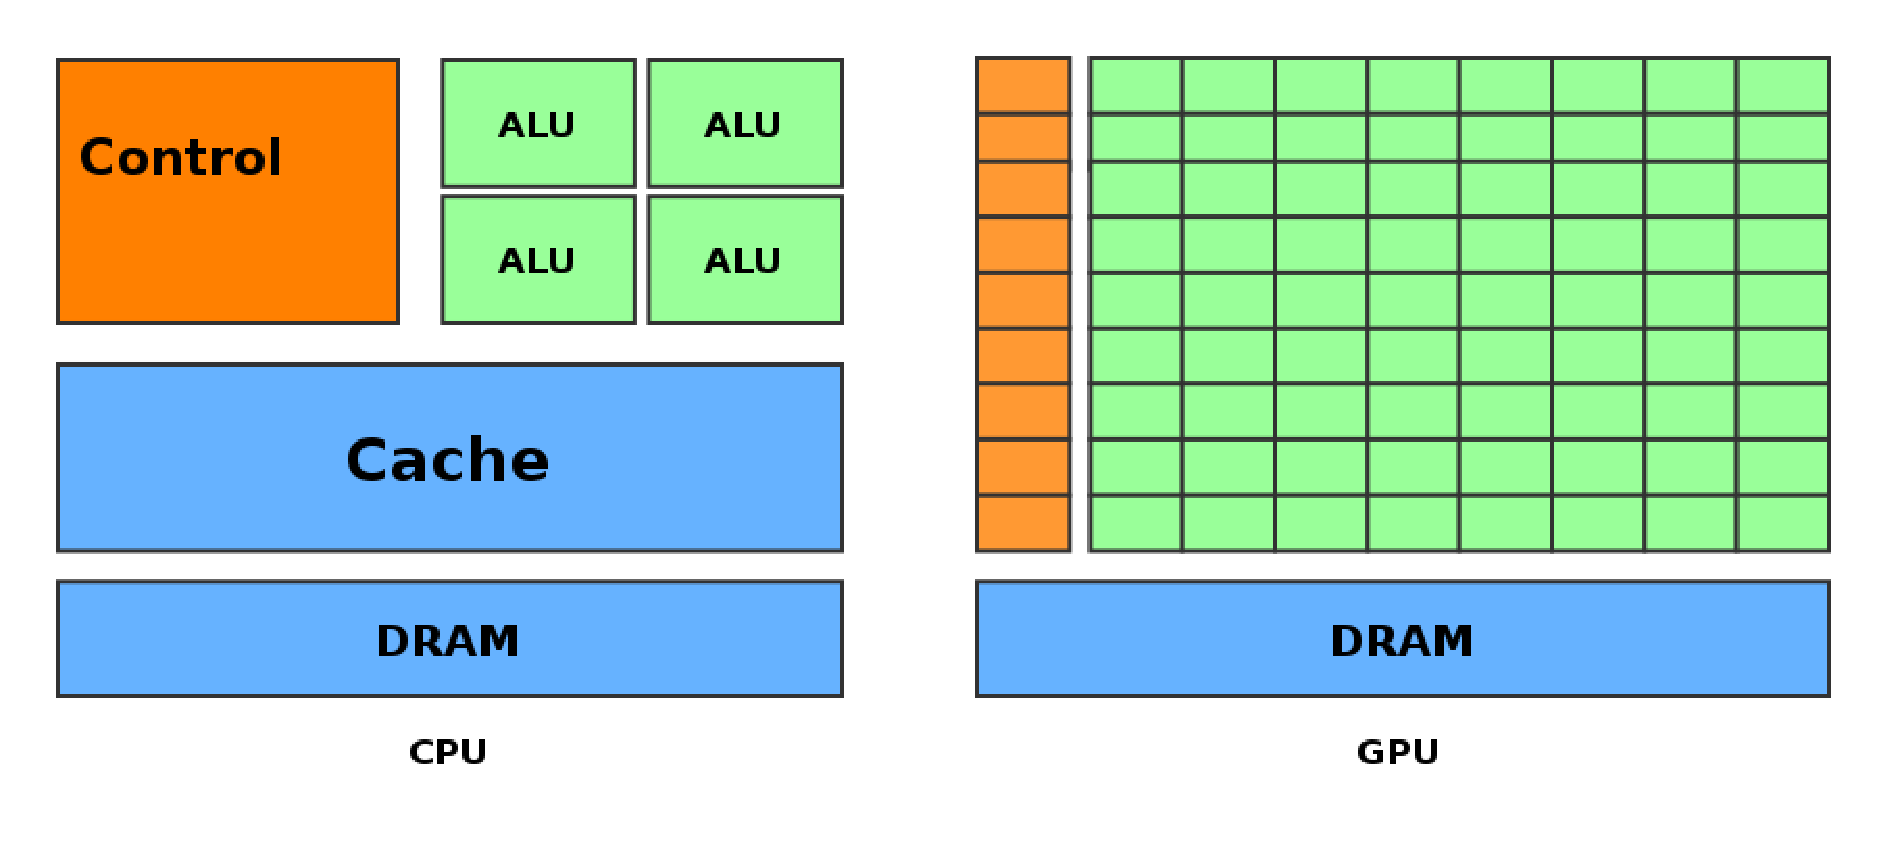
\includegraphics[width=0.9\linewidth]{figure1.eps}
\caption{CPU和GPU结构比较}\label{figure1}
\end{figure}





\chapter{相关技术的研究使用}
本章主要介绍了一些已有的CPU/GPU异构计算优化方法和编译原理中一些调整代码序列的方法,
通过对已有的优化方法进行总结比较,提出本文一种基于代码移动来迁移、合并核函数的数据交换
操作的优化方法。

\section{GPU编程优化方法}
GPU的物理结构更加适合大数据、高并发的复杂计算,任何优化GPU编程的方法都是基于GPU物理
特性充分发挥GPU计算性能来实现的。本节将介绍、对比一些业界主流的GPU编程优化方法以及
每种方法的使用场景。

\subsection{向量化}
\begin{figure}
\centering
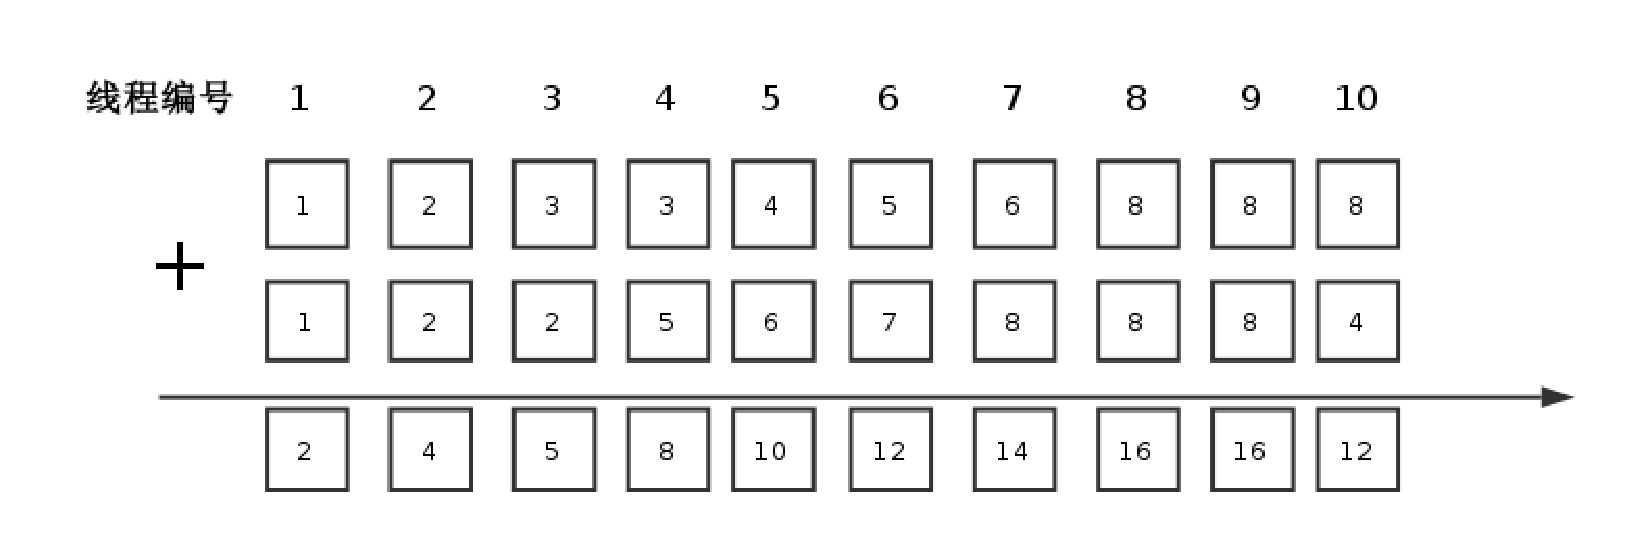
\includegraphics[width=0.9\linewidth]{figure3.eps}
\caption{向量化}\label{figure3}
\end{figure}
程序员可以在编写代码之前手动分析GPU应用程序中数据特点,再根据GPU结构特性去确定如何组织、存储、访问
数据以及确定程序逻辑可以达到优化程序的目的。向量计算是图像算法中经常使用的计算方法,我们可以使用
数组很好地表示一维向量进行计算。但是在向量乘法、加法等计算操作中,向量中每一个维度的操作基本都是相同
而且相互不干扰的,具有很高的并行性。核函数中使用数组表示一维向量时,在向量计算中仅仅使用了
单个线程循环迭代处理向量中每个维度的计算,没有利用到向量的计算并行性和GPU的多核特点,效率较低。
主流GPU编程语言CUDA和OpenCL都提供了数据向量化方法,用专有的数据结构去表示向量。如图~\ref{figure3}所示,向量化后的计算,
每一个维度的的操作都会分配到不同核心上的
线程执行,不再是整个向量维度的计算都在一个线程上。
向量化的数据结构在GPU中计算时可以充分利用GPU多核特性
,每一个维度的计算都放在了不同核心上的线程,可以加速向量计算。

\subsection{优化GPU内存使用}
第一章简单描述了GPU内存结构,较为复杂,由常量内存、
纹理内存、共享内存和全局DRAM等组成。不同种类的存储器特点和适用场景差别很大,表~\ref{table1}
简单列出了不同GPU储存器的一些特点,GPU程序员必须要清楚地了解
GPU的内存特点再根据使用场景具体选择。
编写代码时,如何设计数据在GPU内存中的存储方式也是一种很重要的优化GPU程序的方法。
寄存器是GPU计算单元访问延迟最低的存储器,GPU程序运行时会自动将一些中间数据存储到
寄存器上加速下次读取。但是GPU会将一些线程私有变量存到线程的寄存器上,程序员定义了过多的线程私有变量
会导致程序运行时一些GPU线程内寄存器不足,换而使用显卡中的局部内存,增加了访问延迟。
我们可以把GPU运行时不发生变化的数据存储到GPU常量内存中,单个线程对
常量内存中数据的访问会使GPU将该数据广播到同一线程束中的其他线程,由此可以减少整个程序对常量内存
的读取次数。
\begin{table}[b]
  \centering
  \caption{GPU内存特性}
  \begin{tabular}{llll}
    \hline
    存储器     & 位置      & 访问权限 & 变量生存周期    \\
    \hline
    寄存器     & GPU片上   & GPU可读/写  & 与线程相同    \\
    局部存储器 & 板载显卡  & GPU可读/写  & 与线程相同    \\
    共享内存   & GPU片上   & GPU可读/写  & 与线程块相同   \\
    常量内存   & 板载显卡  & CPU/GPU可读/写  &  与程序相同     \\
    纹理内存   & 板载显卡  & CPU/GPU可读/写  &  与程序相同         \\
    全局内存   & 板载显卡  & CPU/GPU可读/写  &  与程序相同  \\

    \hline
  \end{tabular}
  \label{table1}
\end{table}
共享内存是GPU片上线程块内所有线程可以读写的共享存储空间,是线程块内线程数据交互延迟最低的通信方式。
当程序中一些数据是线程块内所有线程共享的,我们可以使用共享内存代替全局内存,降低线程之间相互通信的延迟。
纹理内存也是GPU中只读内存,被设计用来存储空间局部性比较高的数据。由于GPU结构中没有
cache来缓存时间局部性的数据,如何利用好数据的空间局部性就是一个很重要的优化方法。特别是在图形计算中
,每个像素点的在空间上的联系非常紧密,空间复杂度很高,使用纹理内存的读取特性可以很容易读取空间上联系
紧密的数据,加速内存访问速度。
%CUDA和OpenCL都提供了纹理内存的使用接口,程序员可以根据具体应用数据访问的空间局部性决定是否使用纹理内存。
综合本小节的描述可以看出,GPU中不同内存的性质差别很大,根据具体场景选择
合适的存储器将会很大程度上优化GPU程序。

\subsection{嵌套循环展开}
\begin{lstlisting}[label=Listing1,caption=嵌套循环,language=C++, keywordstyle=\color{blue!70},commentstyle=\color{red!50!green!50!blue!50},frame=shadowbox, rulesepcolor=\color{red!20!green!20!blue!20}] 
void addmatrix(vector<vector<int>>& matrix)
	{
	    int m = matrix.size();
        int n = matrix[0].size();
        for(int i=0; i<m; i++)
            for(int j=0; j<n; j++)
                matrix[i][j] += 1;
        return;
    }		
\end{lstlisting}

\begin{lstlisting}[label=Listing2,caption=嵌套循环展开,language=C++, keywordstyle=\color{blue!70},commentstyle=\color{red!50!green!50!blue!50},frame=shadowbox, rulesepcolor=\color{red!20!green!20!blue!20}] 
void addmatrix(vector<vector<int>>& matrix)
	{
	    int m = matrix.size();
        int n = matrix[0].size();
        for(int i=0; i<m*n; i++)
            {
			    int j = i/n;
			    int k = i%n;
                matrix[j][k] += 1;
			}
        return;
    }		
\end{lstlisting}
GPU之所以能够快速处理大数据并行计算是因为其拥有很多个计算核心,可以同时运行多个线程。GPU程序中的核函数都是
一些计算量很大的循环结构,循环结构中每一次迭代都是独立的,这样GPU就可以启动很多个线程去运行循环结构中的每一次
迭代计算。由此可见,循环结构的迭代次数越多,加速效果越明显。但是GPU程序中循环不都是简单的单层循环,更常见的是
逻辑比较复杂的多层嵌套循环。
在核函数里的多层嵌套循环结构中,只有最里层的循环结构是同时在不同线程上计算的。这样的计算方式使得
嵌套循环结构没有完全利用GPU的多核优势,闲置了很多计算资源。
嵌套循环展开是指预处理GPU程序时把一些核函数中的二层或者多层嵌套循环展开、合并成单个循环。
如代码块~\ref{Listing1}、~\ref{Listing2}所示两段代码都是实现了一个矩阵所有元素加1的简单操作。显然两段代码的时间复杂
都是相同的,嵌套展开后的代码段还增加了计算举证行、列索引的操作。如果在普通CPU上执行的话,显然代码块~\ref{Listing1}
中的代码段执行的会更快,因为CPU是没有足够的计算单元来开启多个线程并行计算该循环的。但是GPU的多核特性正是针对
处理并行程度高的计算的,代码块~\ref{Listing2}把代码块~\ref{Listing1}中的嵌套循环合并成一个迭代比较大的单个循环,这样允许
GPU开启更多的线程去计算该核函数,得到更好的优化效果。这里只拿矩阵自加作为例子介绍嵌套循环展开,当计算比较复杂,
每一次迭代的计算量都比较大时,嵌套循环展开对GPU核函数的优化将是十分明显的。


\subsection{线程配置}
本小节以CUDA平台为例简单描述GPU编程中的线程配置。CUDA的线程设计以网格(Grid)、线程块(Block)和线程(Thread)组成,
具体结构如图~\ref{figure6}所示。GPU上所有的计算单元被划分为两到三个网格,每个网格包含一定数量的线程块,目前
最多为65535个线程块,每个线程块再由一定数量的线程组成,目前主流显卡线程块最多可以包含1024个线程。如何配置好
如此多的线程对GPU程序员将是一个很大的挑战,也是优化GPU程序一个很重要的维度。同一线程块内的线程具有相同的指
令地址,不但能够并发执行,而且可以通过GPU片上共享内存和栅栏实现块内快速通信。这样,程序员在设计CUDA程序时需要
优先把相互通信量较大、较为频繁或者需要同步的线程分配到同一线程块内,利用共享内存降低线程通信延迟,同时把不需
要通信的线程分配到不同线程块内,使其并行粒度更高。CUDA架构通过块间粗粒度并行,块内细粒度并行两种方式来组织线程。
多个计算单元加上一些寄存器和共享存储器组成一个多元处理器。每个线程块最终都是交给一个多元处理器执行的。
\begin{figure}
\centering
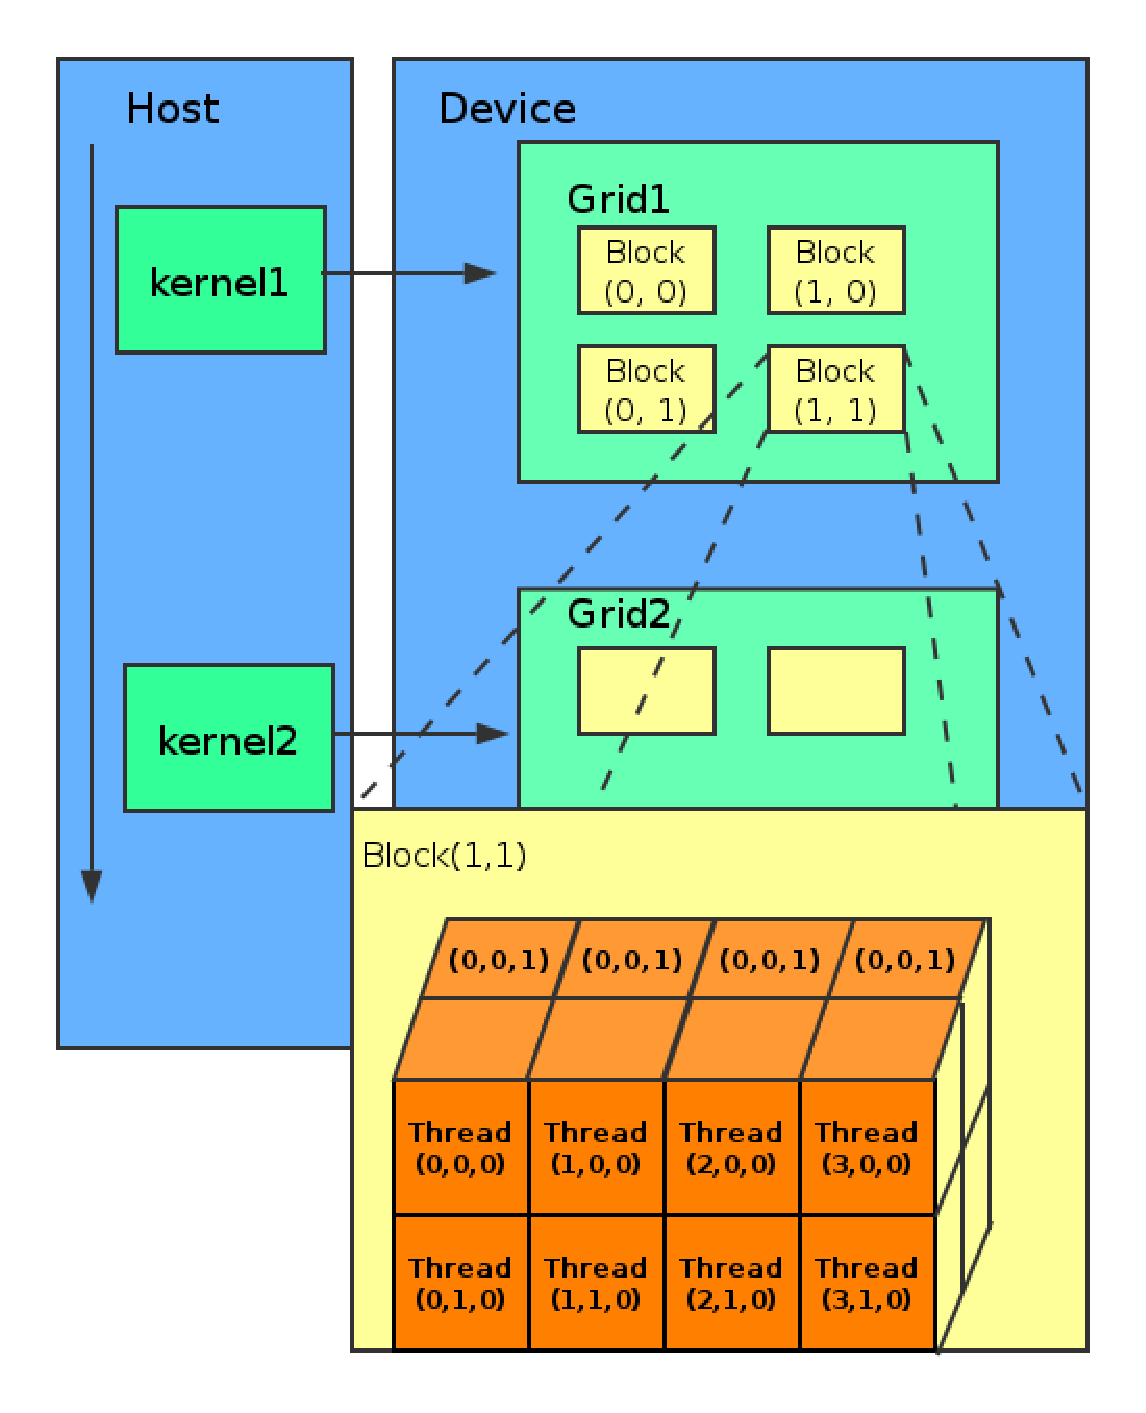
\includegraphics[width=0.6\linewidth]{figure6.eps}
\caption{GPU线程结构}\label{figure6}
\end{figure}
程序运行时,GPU任务分配单元将网格分配到GPU芯片上。CUDA平台启动时,需要将网格配置信息从CPU下发到GPU,
任务分配单元依据配置信息将线程块块分配到多元处理器上。任务分配单元采用轮询策略:轮询遍历多元处理器有没有足够的资源
来执行新的线程块,如果有则给多元处理器分配一个新的线程块。决定是否成功分配的条件有:块运行时需要的寄存器数量,
共享存储器数量,以及其它的一些限制条件。任务分配单元在任务分配中保持公平,然而我们可以通过手动编程设置块内线程数量,
线程使用的寄存器数和共享存储器数来间接控制,保证处理单元负载均衡。任务以这种方法分配使程序具备了很大的可扩展性:
由于每个子任务都能在任意一个多元处理单元上执行,CUDA程序在核心数量不同的处理器上都能正常运行,隐藏了硬件差异。
程序员需要根据具体应用场景将任务拆分为互不相干、可以并行计算的粗粒度子任务,再将每个子任务拆分为能够尽可能利用
线程块内计算资源、存储资源的细粒度指令集。
现有的显卡同一时刻只能执行一个核函数,但是在Fermi架构中可以在同一时刻运行多个核函数。
例如程序员可以在一个内核访问GPU数据的同时,开启另一个内核进行计算,可以很大程度上提高程序运行效率。
线程是串行执行指令的,这就要求每个线程不可以有过多的循环逻辑或者需要过多的存储资源。
当然我们也不应该在单个线程块内分配过多的线程,可能由于参数和中间变量过多导致存储资源不足,降低多元处理器计算速度。
在问题相对复杂时,程序员也可以手动测试一些配置参数的运行速度,选择一个最合适的线程配置参数。

\section{一般代码优化}
程序员编写的代码不总是十全十美,编译器可以自动在不改变程序运行效果的前提下帮助我们进行一些代码优化,使之运行时
的空间效率和时间效率得到提高。编译原理中的代码优化是指通过重排、删除、合并或改变程序片段等策略,使程序代码发生
形式上的改变。本节讨论的是编译阶段的一些代码优化方法,不考虑程序本身算法的效率。
\subsection{变量优化}
任何一个程序离不开变量的定义和变量计算,一些基于变量的简单优化方法可以起到一定的优化效果。表~\ref{table2}给出了
常量合并的传播的优化方法,在编译时就已经可以计算出的常量不需要放到程序执行时计算,减少程序运行时间。
\begin{table}[h]
  \centering
  \caption{常量合并与传播优化}
  \begin{tabular}{p{7cm}<{\centering}p{7cm}<{\centering}}
    \hline
    优化前代码     & 优化后代码   \\
    \hline
    X = 3;         & X = 3;    \\
    Y = X + 2;       & Y = 5; \\
    Z = 3 * Y;      & Z = 15; \\
   \hline
  \end{tabular}
  \label{table2}
\end{table}
表~\ref{table3}描述了公共子表达式外提的优化实例,把两个表达式中重复出现的部分外提出来单独运算,显然优化前
进行了4次加法,优化后进行了3次加法,可以起到一定的加速作用。
\begin{table}[h]
  \centering
  \caption{公共字表达式外提优化}
  \begin{tabular}{p{7cm}<{\centering}p{7cm}<{\centering}}
    \hline
    优化前代码      & 优化后代码   \\
    \hline
    x = b+c+d;      & t = b+c;    \\
    y = b+c+e;      & x = t+d; \\
                    & y = t+e; \\
   \hline
  \end{tabular}
  \label{table3}
\end{table}
还有一些变量优化的场景,比如编译原理中描述的死代码删除。死代码删除是指某个变量的两次定值之间程序没有对该变量的引用,这说明
变量的第一次赋值是多余的,可以删除。一些无用转移语句可以导致一些分支在编译的时候就确定了是否执行,这样编译器可以在编译的时候
就丢弃这些转移逻辑,提升代码执行速度。
\subsection{循环优化}
循环逻辑是程序中重复执行的代码块,对循环结构的优化将会带来更加显著的优化效果。将循环中的不变量或者不变代码外提是最简单的循环优化
方法。表~\ref{table4}中将循环中的不变量2*x+1提出循环外之后,避免了每次迭代时对2*x+1表达式的计算,优化后只需在循环开始之前计算一次,
大大减少了程序运行时间。
\begin{table}[h]
  \centering
  \caption{循环不变量外提}
  \begin{tabular}{p{7cm}<{\centering}p{7cm}<{\centering}}
    \hline
    优化前代码             & 优化后代码   \\
    \hline
    x = c;                    & x = c;    \\
    for(i=0; i<100; i++)      & t = 2*x+1; \\
      array[i] = 2*x+1;       & for(i=0; i<100; i++) \\
	                          &    array[i] = t;  \\
   \hline
  \end{tabular}
  \label{table4}
\end{table}
将循环体内的运算强度削弱也是一种循环优化的方法,在表~\ref{table5}中,我们在循环体内使用加法代替乘法并且得到相同的计算结果。
这种逻辑上的更改不但没有破坏程序结果,而且将每次迭代中的乘法换成了计算强度相对较小的加法,这种优化的效果将随着循环体执行
次数的增加而增加。
\begin{table}[h]
  \centering
  \caption{循环内运算强度削弱}
  \begin{tabular}{p{7cm}<{\centering}p{7cm}<{\centering}}
    \hline
    优化前代码             & 优化后代码   \\
    \hline
    for(i=0; i<100; i++)      & t = 0; \\
       t = i*5;                & for(i=0; i<100; i++)\\ 
                             &    t += 5;\\
  \hline
  \end{tabular}
  \label{table5}
\end{table}












\chapter{基于优化CPU和GPU内存交互的设计和实现}
前两章总结了大数据高通量仿真中CPU/GPU异构并行计算的必要性和一些已有的GPU异构编程优化方法,并利用编译
原理中引用-定值链和定值-引用链分析程序中的数据流,介绍了一些适用于一般程序的代码移动优化方法。
程序员只有清楚的了解CPU/GPU的体系结构特点,再根据具体的应用场景设计合适的程序逻辑,选择合适的GPU编程
优化方法才能够编写出充分利用GPU计算性能的程序。本章基于CPU/GPU异构计算的内存隔离特点,结合编译原理中的代码
移动规则新提出了一种通过修改源代码来减少CPU和GPU内存之间数据交换带来的系统消耗的优化方法,并在第四章
通过一些对比实验证明了本文提出的方法确实有优化GPU程序的作用。
\section{迁移数据交换操作}
由于CPU和GPU的内部结构不同,CPU适合处理顺序计算、程序逻辑以及系统IO等任务,而GPU适合处理高度并行的复杂计算任务。
所以在CPU/GPU异构体系结构中运行的程序包含CPU代码、GPU代码以及CPU和GPU的交互代码。
普通的程序逻辑就是CPU代码,CPU和GPU内存之间的数据交换操作就是交互代码,核函数就是由GPU代码组成的。
CPU内存和GPU内存是隔离的,运行CPU代码时我们把需要的所有数据拷贝到GPU内存中,同样地运行GPU代码时,我们需要把所有数据拷贝
到GPU内存中。所以GPU程序中每一次核函数的调用,通常会在CPU内存和GPU内存之间进行两次数据交换。核函数执行之前,
CPU和GPU执行相应的交互代码API(CudaMalloc、CudaMemcpy)在GPU内存分配相应大小空间并把核函数需要的数据拷贝到GPU已分配
内存中,这个过程称为数据拷入操作(data copyin)。data copyin操作结束之后,GPU开始启动运行核函数(execution)。
在核函数计算结束之后,我们需要把GPU中计算的结果再次拷贝到CPU内存,称为数据拷出(data copyout)。最后如果GPU
中的变量不会再被后续核函数使用,GPU会释放核函数运行之前分配的GPU内存,这是数据释放操作(data freeing)。
由此可见数据在CPU和GPU内存交换的总时间是由一下三个部分组成的:1.在GPU内存上分配空间等预处理操作时间;
2.数据在PCIe总线上传输时间;3.GPU释放内存等清理操作时间。在核函数比较多的程序中,CPU和GPU之间频繁的数据交换
将成为整个程序的瓶颈,这也是本文优化方法的出发点。本节主要是根据编译原理中代码移动原理迁移GPU程序中核函数的数
据拷贝操作,使原来在程序中固定点执行的数据交换操作可以允许在程序中的一段代码区间执行。
\subsection{迁移限制}
如上所述,一个核函数的执行被拆分成了四个独立的阶段,数据拷入, 执行, 数据拷出和数据释放。
显然这四个阶段的执行顺序是不能颠倒的,必须按照数据拷入$\rightarrow$执行$\rightarrow$数据拷出$\rightarrow$数据释放
的顺序执行,但是每个操作具体的执行时间确是可以调整的。本文的出发点是优化数据交换操作,所以我们不迁移核函数的执行
操作,只迁移数据拷入,数据拷出,数据释放三个数据交换操作。我们可以把数据拷入操作的交互代码可以看作是CPU代码中对变量的一个引用,可以沿着
代码语句序列向上移动直到程序中某个点改变了该数据,即遇到该变量的定值点就不能再向上移动了,同时我们得保证数据拷入操作
在核函数开始执行之前完成。同样地,我们也可以把交互代码中的数据拷出操作看作是CPU代码中队变量的定值,可以和数据释放操作一起
沿着代码语句序列向下移动,直到程序中出现某条语句引用该变量,即遇到该变量的引用点结束,同时我们必须保证数据
拷出和数据释放操作是在核函数执行完成之后才开始执行的。数据拷出操作之后,为了减少GPU内存的占用,我们将立刻释放相应的GPU内存,
除非该内存数据会在后续的核函数中继续用到我们才选择继续保存,这样可以减少冗余的数据拷贝。
所以在整个数据交换操作的迁移过程中数据依赖性是迁移的前提,
在下面的章节我们将利用编译原理中的引用-定值链和定值-引用链方法来分析
整个程序中的控制流和数据流,得到具体的迁移操作。
\subsection{代码移动}
现在我们介绍如何调整核函数执行过程中的四个阶段,以及如何根据代码移动方法迁移核函数的数据交换操作。
代码块~\ref{Listing4}描述了原始CUDA代码中一个核函数的结构,数据拷入操作,核函数执行,数据拷出操作,以及数据释放操作
是一个紧密的整体。但是在代码块~\ref{Listing5}中,数据拷入操作被提前执行,同时数据拷出和数据释放操作被推后执行。
显然代码块~\ref{Listing5}中针对数据操作的迁移并没有改变代码块~\ref{Listing4}中的执行结果。
本文的GPU程序优化算法只针对CPU和GPU内存之间的数据交换操作,所以我们只迁移数据交换操作。
\newpage
\begin{lstlisting}[label=Listing4,caption=原始CUDA代码,language=C, keywordstyle=\color{blue!70},commentstyle=\color{red!50!green!50!blue!50},frame=shadowbox, rulesepcolor=\color{red!20!green!20!blue!20}] 
__global__ void kernel(int *device, int i);
int host[1000] = {0}, tmp[1000] = {0};
for (int i = 0; i < 1000; i++)
    host[i] = host[i] + 1;
......
for (int i = 0; i < 1000; i++)
    tmp[i] = tmp[i]+1;
int *device;
CUDAMalloc(&device, sizeof(int) * 1000);
CUDAMemcpy(device, host, sizeof(int) * 1000,CUDAMemcpyHostToDevice); /*data copyin*/
for (int i = 0; i < 1000; i++) /*execution*/
    kernel<<<1,1>>>(device, i);
CUDAMemcpy(host, device, sizeof(int)* 1000,
CUDAMemcpyDeviceToHost); /*data copyout*/
CUDAFree(device); /*data freeing*/
......
for (int i = 0; i < 1000; i++)
    tmp[i] = tmp[i]+1;
\end{lstlisting}

\begin{lstlisting}[label=Listing5,caption=迁移数据拷贝操作,language=C, keywordstyle=\color{blue!70},commentstyle=\color{red!50!green!50!blue!50},frame=shadowbox, rulesepcolor=\color{red!20!green!20!blue!20}] 
__global__ void kernel(int *device, int i);
int host[1000] = {0}, tmp[1000] = {0};
for (int i = 0; i < 1000; i++)
    host[i] = host[i]+1;
int *device;
CUDAMalloc(&device, sizeof(int) * 1000);
CUDAMemcpy(device, host, sizeof(int) * 1000, CUDAMemcpyHostToDevice); /*data copyin*/
......
for (int i = 0; i < 1000; i++)
    tmp[i] = tmp[i]+1;
for (int i = 0; i < 1000; i++) /*execution*/
    kernel<<<1,1>>>(device, i);
......
for (int i = 0; i < 1000; i++)
    tmp[i] = tmp[i]+1;
CUDAMemcpy(host, device, sizeof(int)* 1000,
CUDAMemcpyDeviceToHost); /*data copyout*/
CUDAFree(device); /*data freeing*/
\end{lstlisting}
核函数的数据拷入操作可以沿着代码语句序列向上移动,我们只要保证数据拷入操作在相应数据的定值点之后和核函数执行之前的代码区间执行就是合法的。
同样数据拷出操作可以沿着代码语句序列向下移动,我们只要保证数据拷出操作在相应数据的引用点之前和核函数执行之后的代码区间执行就是合法的
至于核函数的数据释放操作,必须保证在数据拷贝操作之后执行。当程序在GPU上内存使用量较少而且GPU内存足够使用时,我们可以选择让GPU内存保持所有的
数据直到整个程序执行结束之后释放。但是GPU内存在使用时不总是足够的,所以我们选择在数据拷出到CPU内存之后立刻让GPU内存释放该变量,除非该变量
在后续核函数中会再次用到才让GPU内存保持。
\subsection{异步操作优化}
\begin{figure}[h]
\centering
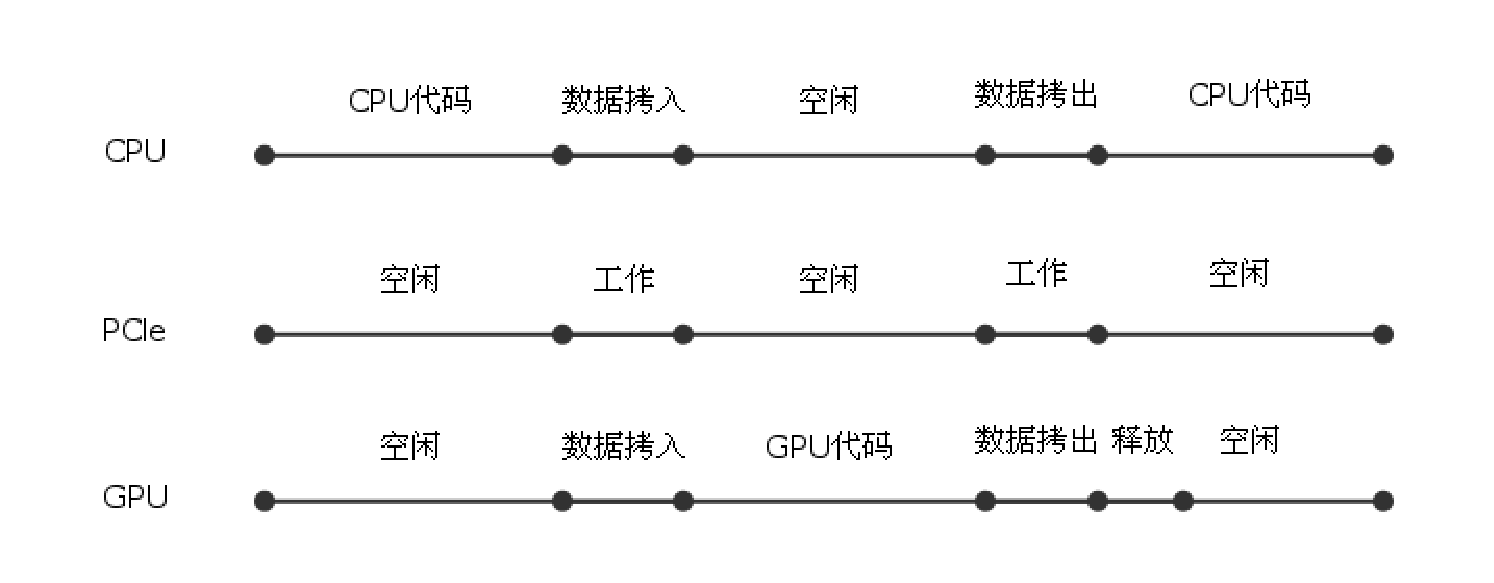
\includegraphics[width=1\linewidth]{figure9.eps}
\caption{初始结构}\label{figure9}
\end{figure}
\begin{figure}[h]
\centering
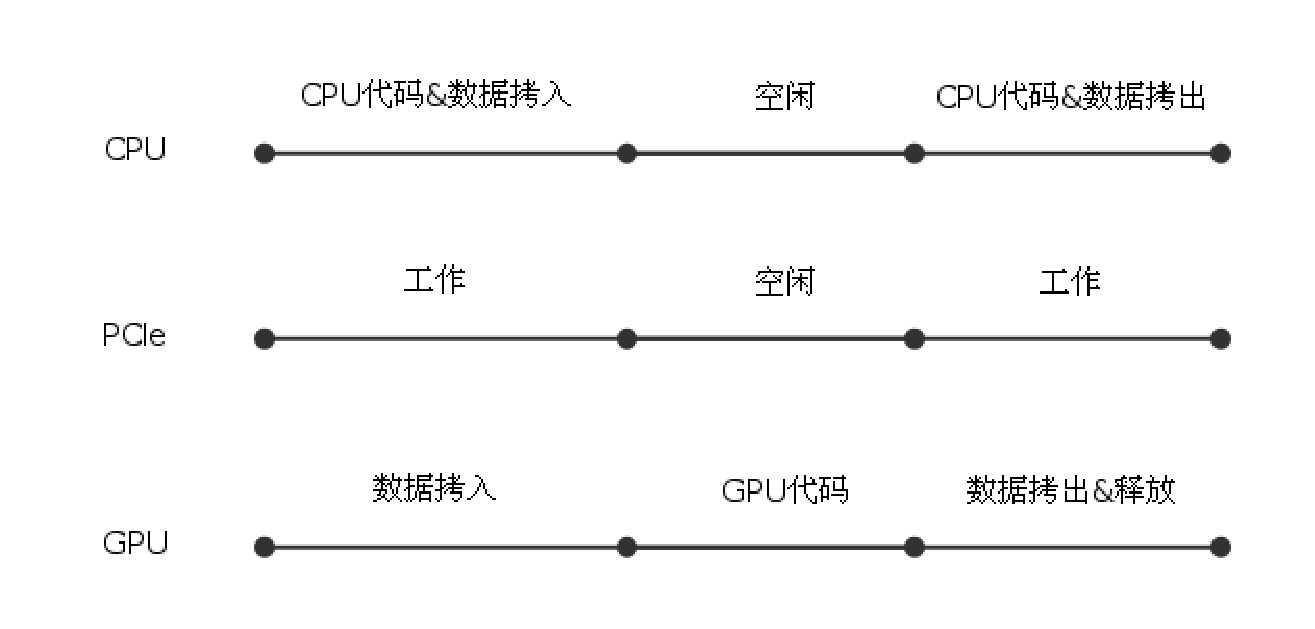
\includegraphics[width=1\linewidth]{figure10.eps}
\caption{异步优化}\label{figure10}
\end{figure}
这里先单独讨论一下单个核函数在数据拷贝操作迁移之后的异步优化。我们发现数据拷入操作沿着代码序列向上移动之后,数据拷入操作和核函数执行的代码语句之间
出现了一部分CPU代码。同样地,数据拷出操作沿着语句序列向下移动之后,核函数结束执行和数据拷出操作之间也有一部分CPU代码。我们再迁移数据交换操作时是以
数据依赖性为前提的,所以这部分CPU代码和数据交换操作时没有任何依赖的,即可以异步并行执行。图~\ref{figure10}对图~\ref{figure9}中单个核函数的
执行过程进行了一些异步优化。首先在图~\ref{figure9}中第一段CPU代码执行时,PCIe和GPU都处于空闲状态,数据拷入操作在CPU代码完全执行结束之后才开始。
我们在代码块~\ref{Listing5}中可以看到,在迁移数据拷入操作之后,又一块CPU代码可以和数据拷入操作异步执行。CPU代码执行时不占用PCIe总线和GPU资源,
GPU预分配内存和数据拷入操作也不占用CPU代码执行时需要的计算资源。图~\ref{figure10}中的并行策略可以更加充分地利用CPU/GPU资源和PCIe总线带宽。
同样地,我们也可以对数据拷出操作和CPU代码进行异步优化,这里就不做赘述。
当然如果程序员足够聪明,可以在设计核函数时就选择以异步的方式进行数据拷贝操作。
异步优化必须要有一块与数据交换操作无依赖、可并行的CPU代码时才能发挥作用,这与我们本文提出的减少数据交换频率和数据交换总量的优化方法不相同。





%%==================================================
%% conclusion.tex for BIT Master Thesis
%% modified by yang yating
%% version: 0.1
%% last update: Dec 25th, 2016
%%==================================================


\begin{conclusion}

本文采用……。{\color{blue}(结论作为学位论文正文的最后部分单独排写,但不加章号。结论是对整个论文主要结果的总结。在结论中应明确指出本研究的创新点,对其应用前景和社会、经济价值等加以预测和评价,并指出今后进一步在本研究方向进行研究工作的展望与设想。结论部分的撰写应简明扼要,突出创新性。)}

\end{conclusion}

%% 参考文献,五号字,使用 BibTeX,包含参考文献文件.bib

%\bibliography{reference/chap1,reference/chap2} %多个章节的参考文献
\bibliography{reference/chap1}


%%%%%%%%%%%%%%%%%%%%%%%%%%%%%%
%% 后置部分
%%%%%%%%%%%%%%%%%%%%%%%%%%%%%%

%% 附录(章节编号重新计算,使用字母进行编号)
\appendix
\renewcommand\theequation{\Alph{chapter}--\arabic{equation}}  % 附录中编号形式是"A-1"的样子
\renewcommand\thefigure{\Alph{chapter}--\arabic{figure}}
\renewcommand\thetable{\Alph{chapter}--\arabic{table}}

%%==================================================
%% app1.tex for BIT Master Thesis
%% modified by yang yating
%% version: 0.1
%% last update: Dec 25th, 2016
%%==================================================


\chapter{***}

附录相关内容…
 

\chapter{Maxwell Equations}


因为在柱坐标系下,$\overline{\overline\mu}$是对角的,所以Maxwell方程组中电场$\bf
E$的旋度

所以$\bf H$的各个分量可以写为:
\begin{subequations}
  \begin{eqnarray}
    H_r=\frac{1}{\mathbf{i}\omega\mu_r}\frac{1}{r}\frac{\partial
      E_z}{\partial\theta } \\
    H_\theta=-\frac{1}{\mathbf{i}\omega\mu_\theta}\frac{\partial E_z}{\partial r}
  \end{eqnarray}
\end{subequations}
同样地,在柱坐标系下,$\overline{\overline\epsilon}$是对角的,所以Maxwell方程组中磁场$\bf
H$的旋度
\begin{subequations}
  \begin{eqnarray}
    &&\nabla\times{\bf H}=-\mathbf{i}\omega{\bf D}\\
    &&\left[\frac{1}{r}\frac{\partial}{\partial
        r}(rH_\theta)-\frac{1}{r}\frac{\partial
        H_r}{\partial\theta}\right]{\hat{\bf
        z}}=-\mathbf{i}\omega{\overline{\overline\epsilon}}{\bf
      E}=-\mathbf{i}\omega\epsilon_zE_z{\hat{\bf z}} \\
    &&\frac{1}{r}\frac{\partial}{\partial
      r}(rH_\theta)-\frac{1}{r}\frac{\partial
      H_r}{\partial\theta}=-\mathbf{i}\omega\epsilon_zE_z
  \end{eqnarray}
\end{subequations}
由此我们可以得到关于$E_z$的波函数方程:
\begin{eqnarray}
  \frac{1}{\mu_\theta\epsilon_z}\frac{1}{r}\frac{\partial}{\partial r}
  \left(r\frac{\partial E_z}{\partial r}\right)+
  \frac{1}{\mu_r\epsilon_z}\frac{1}{r^2}\frac{\partial^2E_z}{\partial\theta^2}
  +\omega^2 E_z=0
\end{eqnarray}
 

%(其后部分无编号)
\backmatter

% 发表文章目录
%%==================================================
%% pub.tex for BIT Master Thesis
%% modified by yang yating
%% version: 0.1
%% last update: Dec 25th, 2016
%%==================================================

\begin{publications}{99}

    \item\textsc{高凌}. {交联型与线形水性聚氨酯的形状记忆性能比较}[J].
      化工进展, 2006, 532-535.(核心期刊)
    
\end{publications}

% 致谢
%%==================================================
%% thanks.tex for BIT Master Thesis
%% modified by yang yating
%% version: 0.1
%% last update: Dec 25th, 2016
%%==================================================

\begin{thanks}

本论文的工作是在导师……。

\end{thanks}

% 作者简介(博士论文需要)
%%==================================================
%% resume.tex for BIT Master Thesis
%% modified by yang yating
%% version: 0.1
%% last update: Dec 25th, 2016
%%==================================================

\begin{resume}

本人…。

\end{resume}



\end{document}
